\chapter{Architettura del sistema}\label{ch:chapter9}
L'idea alla base del sistema IoT � quella di progettare una catena di produzione tipica di un'industria 4.0 attraverso l'utilizzo di SDN-Wise. Per lo sviluppo del sistema sono state affiancate le tecnologie di SDN-Wise, approfondite nei capitoli precedenti, con metodologie per effettuare le lavorazioni e monitorare l'andamento della catena industriale con prevenzione per gusti e malfunzionamenti. 
\newline 
Il sistema progettato prevedeva gi� all'interno tutti i meccanismi previsti dal SDN-Wise e sono stati implementati i seguenti meccanismi per la realizzazione finale:
\newline
- \textbf{sondaggio}: per monitorare l'ambiente � stato implementato un sistema di consenso distribuito, nella quale ogni nodo che partecipa al sondaggio comunica con gli altri nodi partecipanti, invece di avere una comunicazione unicast con il Controller.
\newline
- \textbf{attuatori e meccanismo di prevenzione guasti}: per la prevenzione guasti o errore di lavorazione durante la catena industriale sono stati implementati dei meccanismi di allarme e dei nuovi mote che compiessero delle azioni per salvaguardarlo.

\section{Attori partecipanti}
Nel sistema progettato gli attori principali sono tre e partecipano tutti attivamente per la realizzazione della catena industriale con lavorazione e risposta ai guasti e agli errori di lavorazione. In particolare questi tre elementi sono \textbf{Controller}, \textbf{Sink} e  \textbf{Mote}. Di seguito verranno analizzati singolarmente in maniera pi� approfondita. 
\subsection{Controller}
Il Controller � un entit� logica centralizzata, che ha la visione completa e aggiornata della topologia della rete e delle relazioni tra i nodi. Per interfacciarsi con la rete, esso apre una comunicazione TCP con il Sink, attraverso la quale il Controller pu� inviare pacchetti per la modifica della topologia della rete o per riceve pacchetti sullo stato dei nodi o delle richieste da parte di essi. 
\newline 
\begin{figure}[htbp]
\centering
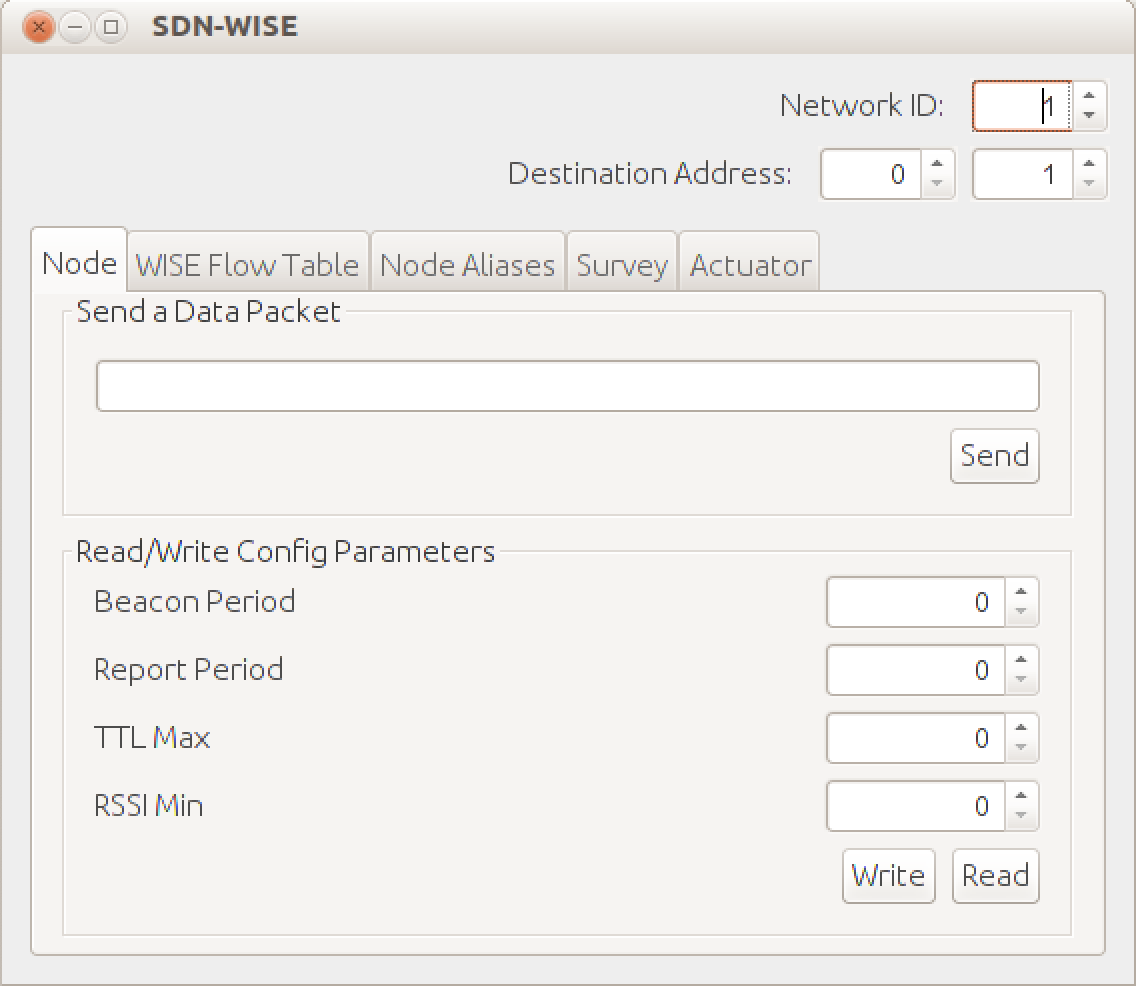
\includegraphics[width=0.60\textwidth,height=\textheight,keepaspectratio]{images/fig_9_1}
\caption{Pannello del Controller}
\label{fig:6_4}
\end{figure}
\newline
Nel sistema progettato il Controller si presenta come nella figura soprastante. Questo pannello da la possibilit� all'Operatore, che ha il compito di monitorare la catena industriale e di avviare le lavorazioni, di inviare pacchetti di vario genere per monitorare il funzionamento dell'intero sistema o per modificare la struttura topologica.
\newline
Per il monitoraggio della rete, nel sistema � previsto un pannello che riproduce la topologia della rete basandosi sui pacchetti dei report, pacchetti nel quale ogni nodo specifica i suoi vicini. Un esempio � mostrato in figura:
\newline
\begin{figure}[htbp]
\centering
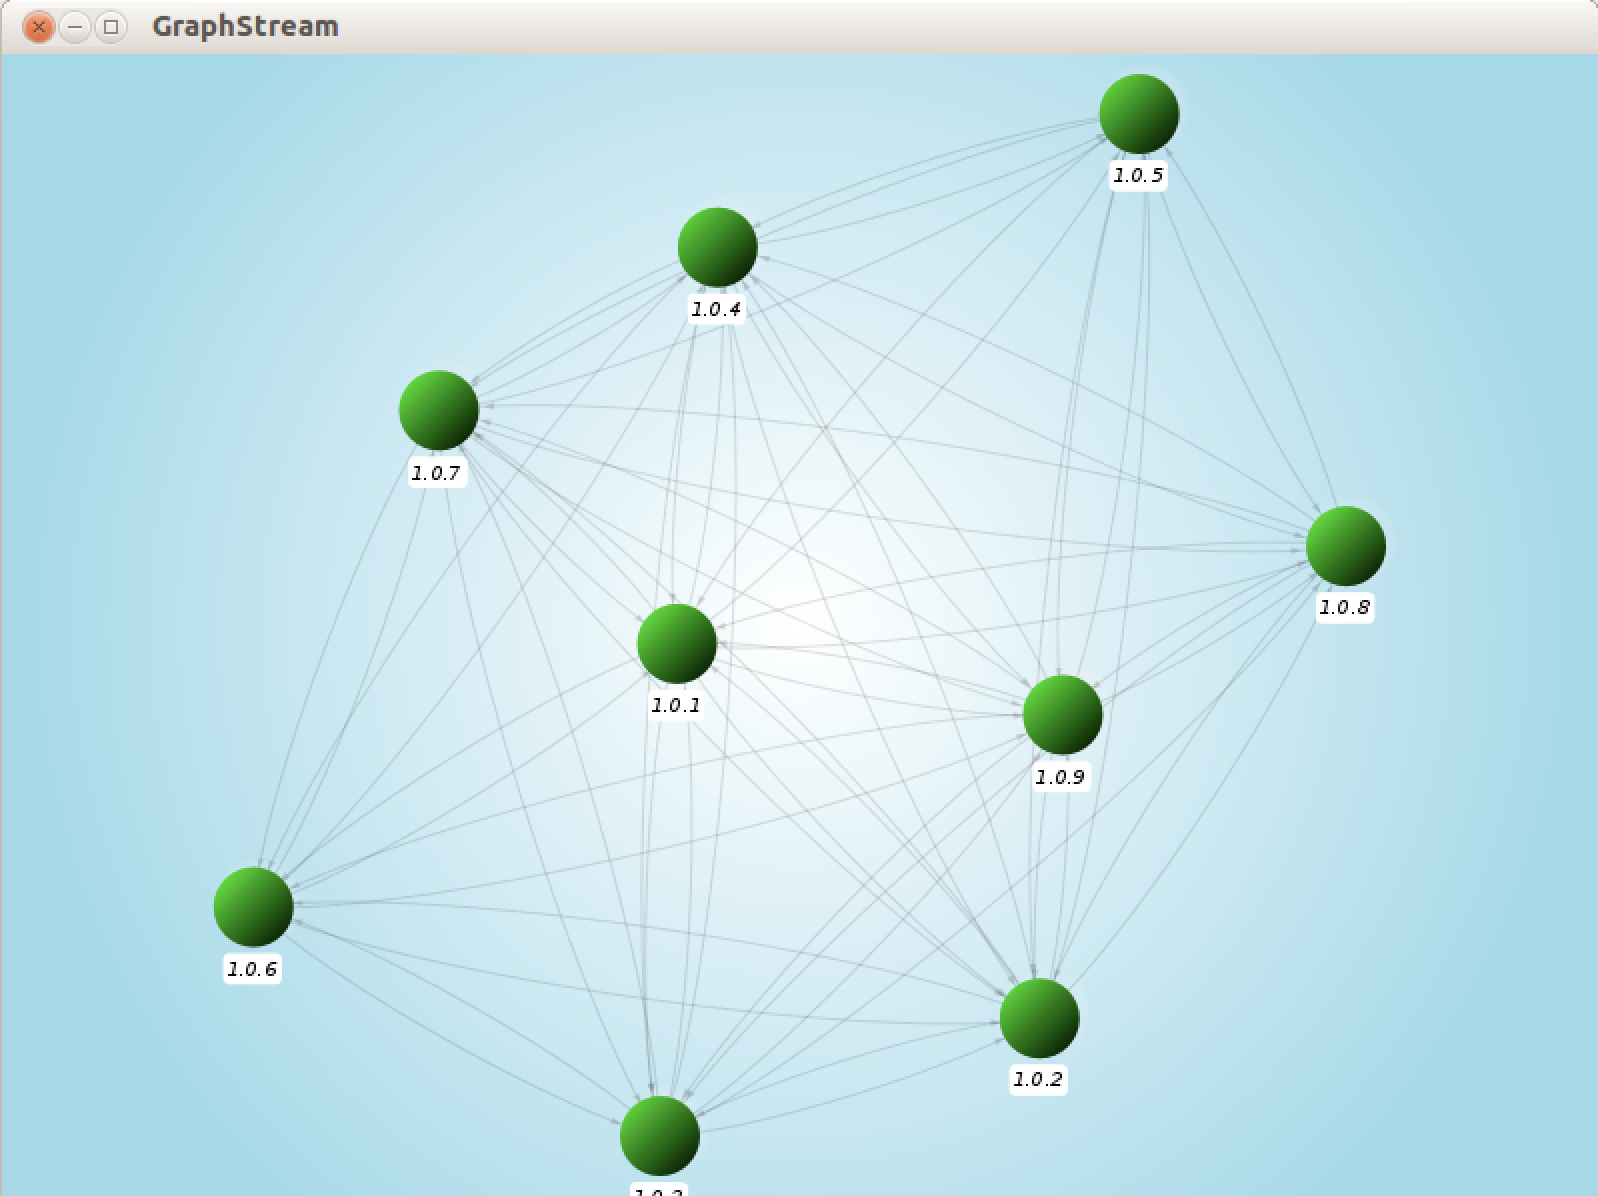
\includegraphics[width=0.70\textwidth,height=\textheight,keepaspectratio]{images/fig_9_2}
\caption{Topologia Rete}
\label{fig:6_4}
\end{figure}
\newline
\subsubsection{Survey e Actuator}
All'interno del pannello del controller sono presenti due campi, Survey e Actuator. 
\newline
\begin{figure}[htbp]
\centering
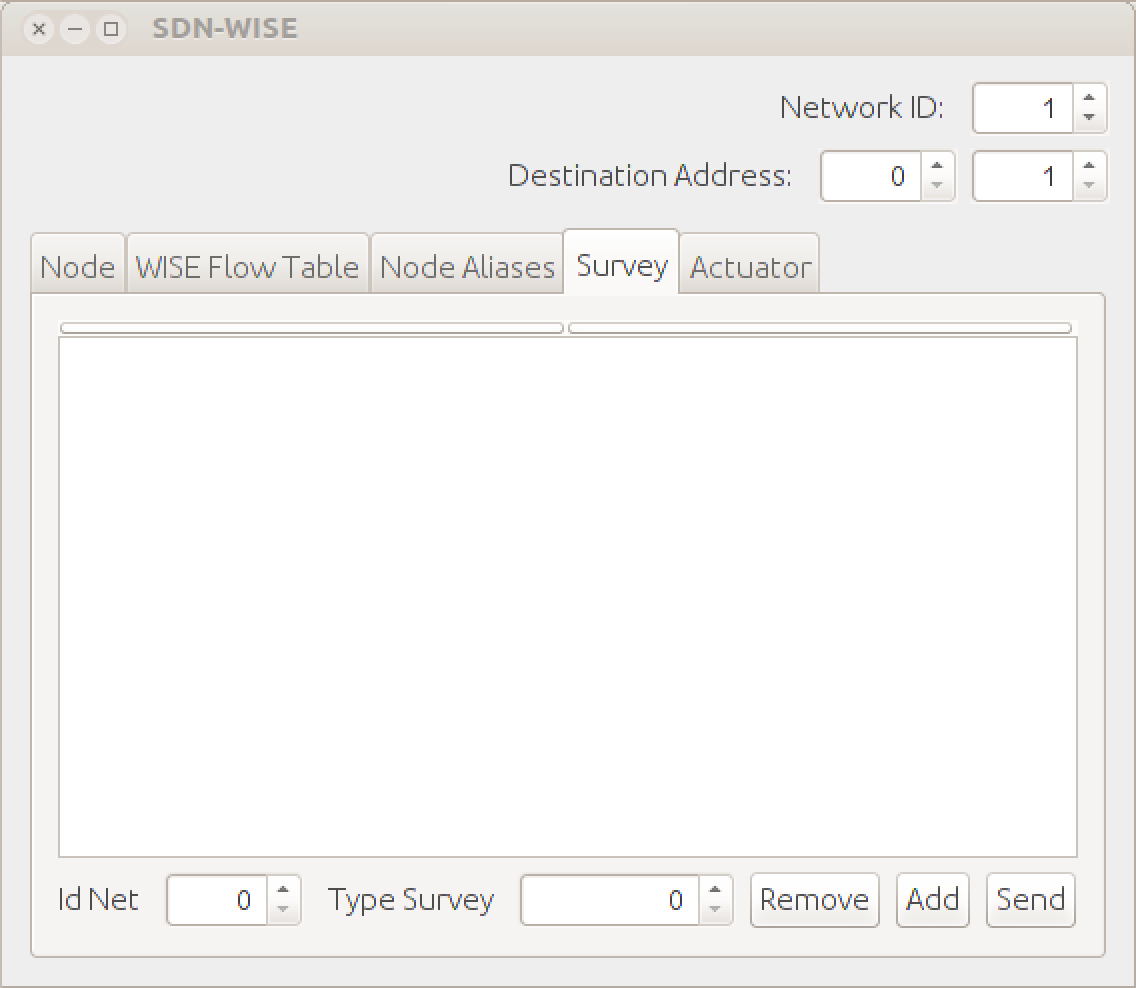
\includegraphics[width=0.70\textwidth,height=\textheight,keepaspectratio]{images/fig_9_1_1}
\caption{Pannello Survey}
\label{fig:6_4}
\end{figure}
\newline
Quest'ultimi presentano una tabella a due colonne che rappresentano rispettivamente l'High Adress e Low Adress degli indirizzi dei nodi che partecipano. I due Spinner in basso al pannello rappresentano ID della rete, che andr� a inserirsi nel primo byte dell'Header, e il TYP(azione o sondaggio), che sar� il primo byte del payload. 
\newline
\newline
Di fianco ai due Spinner, sono presenti tre bottoni, remove, Send e Add; questi tre attivano tre metodi differenti:
\newline
- \textbf{Remove}: rimuove un nodo dalla tabella.
\newline
- \textbf{Add}: inserisce un nuovo nodo nella tabella; per inserirlo, una volta cliccato il pulsante add apparir� il seguente pannello aggiuntivo:
\newline
\newline
\begin{figure}[htbp]
\centering
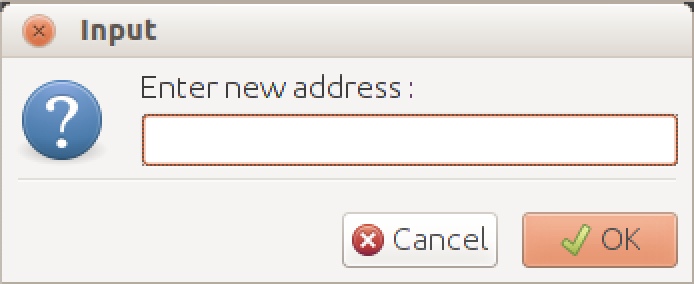
\includegraphics[width=0.60\textwidth,height=\textheight,keepaspectratio]{images/fig_9_1_2}
\caption{Pannello newAddress}
\label{fig:6_4}
\end{figure}
\newline
\newline
- \textbf{Send}: invia il pacchetto al Sink.
\newline
I nodi della tabella, ogni volta che viene compiuto l'evento add, vengono aggiunti a una lista di NodeAdress; premuto il tasto send, invece, viene creata la lista di valori, inizialmente inizializzata a zero, e viene creato il pacchetto per inviarlo al Sink.
\subsection{Sink}
Il Sink � un nodo della rete ed � l'unico nodo che pu� dialogare con il Controller; questo fa si che gli altri nodi della rete conoscano il suo indirizzo in modo tale che tutti possano inviare richieste o report al Controller. Dal Sink passano tutti i pacchetti , questo lo rende il perno fondamentale della rete ed � grazie a lui che il Controller pu� conoscere ogni dettaglio della rete. All'interno del framework \textit{Cooja} il Sink � raffigurato con il colore verde.
\newline
\begin{figure}[htbp]
\centering
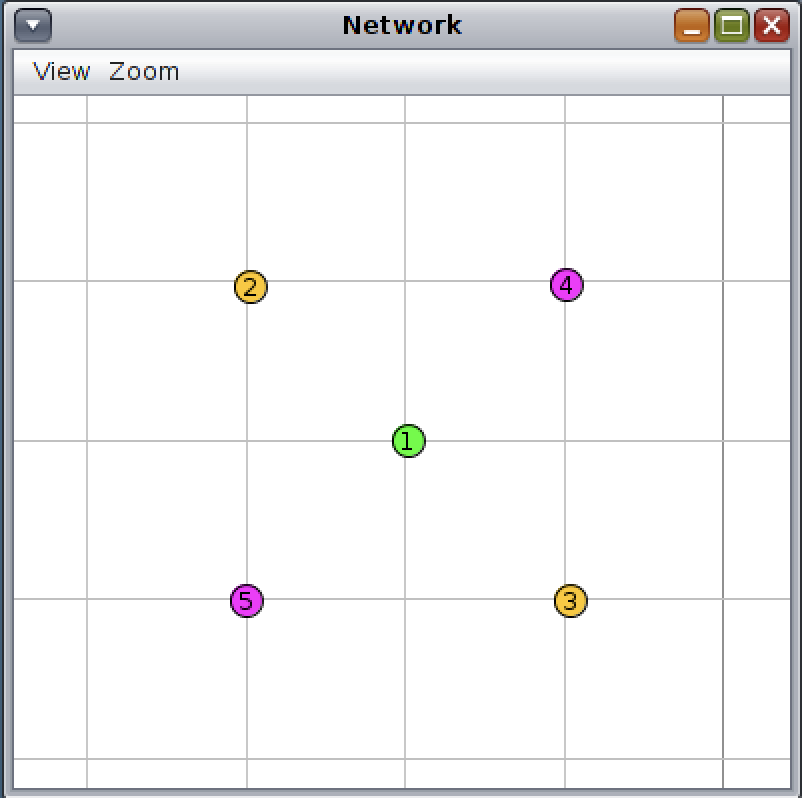
\includegraphics[width=0.60\textwidth,height=\textheight,keepaspectratio]{images/fig_9_3}
\caption{Sink, Mote e Actuator Mote}
\label{fig:6_4}
\end{figure}
\newline
\subsection{Mote}
I mote sono i restanti nodi della rete, i compiti principali sono di dialogare tra loro e con il Sink attraverso l'invio di pacchetti \textit{beacon,report,request}. 
\newline
Nel sistema progettato i mote si dividono in due categorie:
\newline
- \textbf{Mote}: hanno il compito di monitorare l'ambiente, monitorando i dati richiesti dal sondaggio.
\newline
- \textbf{Actuator Mote}: gli Actuator Mote hanno il compito di attuare un'azione specifica per prevenire un danno ambientale.
\newline
All'interno del framework \textit{Cooja} il Mote � raffigurato con il colore giallo, mentre l'Actuator Mote con il colore viola.
